\documentclass[11pt]{article}
\usepackage{jmlr2e}
\usepackage{booktabs}
\usepackage{hyperref}
\usepackage{xcolor}

\hypersetup{colorlinks=true, linkcolor=black, citecolor=black, urlcolor=blue}

\jmlrheading{1}{2026}{1--6}{4/26}{4/26}{Konark}
\ShortHeadings{An Empirical Study of Double Descent in Polynomial Regression}{Konark}
\firstpageno{1}

\title{An Empirical Study of Double Descent\\ in Polynomial Regression}

\author{%
  \name Konark \email itsmekonark@gmail.com \\
  \addr School of Computer Science\\
        Constructor University Bremen\\
        28759 Bremen, Germany
}

\editor{Academic Skills in Computer Science}

\begin{document}

\maketitle

\begin{abstract}
Machine-learning textbooks teach that as a model gets more complex,
its error on new data first goes down and then back up. The result
is a U-shape. This is not the whole story. If you keep adding
parameters past the point where the model fits the training data
exactly, the error often goes \emph{down again}. This is called
\emph{double descent}. I show it with about as simple an experiment
as one can ask for: fitting polynomials to a wiggly curve. With
plenty of training data, I get the textbook U-shape. With little
training data, a sharp spike appears at the point where the
polynomial has just enough wiggles to hit every training point---and
then the error drops a second time as the polynomial keeps growing.
Splitting the spike into bias and variance shows that both blow up
at the same time. Adding even a tiny amount of ridge regularisation
makes the spike disappear.
\keywords{double descent, polynomial regression, bias--variance,
overparameterisation, ridge regression}
\end{abstract}

\section{Introduction}
\label{sec:intro}

Almost every machine-learning class starts the same way. A model
that is too simple cannot capture the truth---it has high
\emph{bias}. A model that is too complex chases random noise---it
has high \emph{variance}. Plot test error against model size and
you get a U: bad on the left, bad on the right, best somewhere in
the middle. This has been the standard story for over thirty
years~\citep{geman1992neural,hastie2009elements}.

The story does not match what people actually do today. Modern
neural networks have millions of parameters and only a few thousand
training examples. They fit the training data perfectly. The
U-shape predicts they should be useless on new data, but in practice
they work very well.

In 2019, \citet{belkin2019reconciling} gave a name to what is really
going on: \emph{double descent}. The error follows the U-shape for
small models. Then it spikes---sharply---at the point where the
model has just enough parameters to fit the training set exactly.
Then it goes down again as the model keeps growing. Researchers
have since seen the same shape in many other kinds of models,
including deep neural networks~\citep{nakkiran2021deep}.

This paper has one small goal: to show double descent in the
simplest setting I could find. No neural networks, no heavy theory.
Just fitting polynomials to a one-dimensional toy problem. The
experiments make three points.
\textbf{(i)}~The choice of basis matters. Plain monomials
$1, x, x^2, \ldots$ blow up numerically for moderate model sizes, so
I use a more stable family.
\textbf{(ii)}~The spike at the threshold is caused by \emph{both}
bias and variance blowing up, not by variance alone as is sometimes
claimed.
\textbf{(iii)}~Even a tiny ridge penalty removes the spike, so
double descent is fragile. All the code, figures, and \LaTeX{}
sources are released alongside this paper so anyone can rerun the
experiments.

\section{Related Work}
\label{sec:related}

The classical bias--variance trade-off is described in any standard
textbook~\citep{hastie2009elements} and was given a famous treatment
in the neural-network setting by~\citet{geman1992neural}.
\citet{belkin2019reconciling} brought double descent to the
attention of the machine-learning community, observing it in random
Fourier features, decision trees, and small neural networks.
\citet{nakkiran2021deep} demonstrated it cleanly in modern deep
networks. For linear models, \citet{hastie2022surprises} now
provide a fairly complete asymptotic theory, and
\citet{nakkiran2020optimal} prove that with the right amount of
ridge regularisation the spike disappears entirely. I do not engage
with this theory mathematically. I just re-derive its qualitative
predictions in a small experiment that anyone can run on a laptop.

\section{Experimental Setup}
\label{sec:setup}

The setup is intentionally simple. There are only three pieces:
data, a model, and a way to fit the model.

\paragraph{Data.} I draw $n$ random points between $0$ and $1$.
The label of each point is a smooth wave plus a bit of Gaussian
noise:
\begin{equation}
  y = \sin(2\pi x) + 0.3\,x + \varepsilon,
  \qquad \varepsilon \sim \mathcal{N}(0, 0.3^2).
  \label{eq:data}
\end{equation}
The test set is $2000$ fresh points drawn from the same recipe.

\paragraph{Model.} Polynomial regression with $p$ features. The
natural choice would be $1, x, x^2, \ldots, x^{p-1}$, but those
columns become almost identical for large $p$ and the math blows up
numerically. I use \emph{Legendre polynomials} instead. These are
just a different family of polynomials that stay numerically
well-behaved as $p$ grows. NumPy provides them out of the box
(\texttt{numpy.polynomial.legendre.legvander}).

\paragraph{Fit.} Standard least squares. When the model has more
parameters than data points ($p > n$), there are infinitely many
fits that pass through every training point. I pick the one with the
smallest coefficients---this is what \texttt{numpy.linalg.lstsq}
returns. Some experiments also add a small \emph{ridge} penalty
$\lambda$ that discourages large coefficients.

\paragraph{Reporting.} I run each experiment many times
($30$--$400$) with fresh random data and report averages or
medians. All random seeds are fixed in the code, so every figure is
bit-for-bit reproducible.

\section{Experiments}
\label{sec:experiments}

\subsection{The classical regime: a tame U-curve}

\begin{figure}[t]
\centering
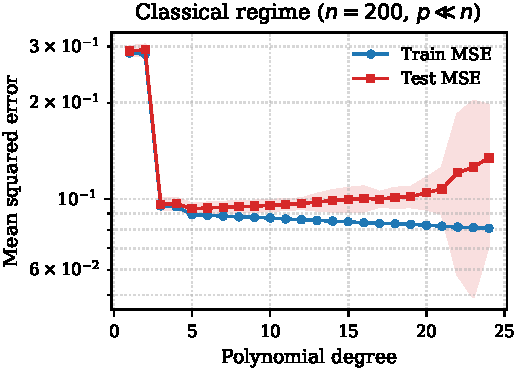
\includegraphics[width=0.55\linewidth]{figures/fig_classical_ushape.pdf}
\caption{Classical U-shaped trade-off. With $n=200$ training points
and polynomial degrees up to $24$ (so $p \ll n$), the test error is
minimised at degree $\approx 5$ and slowly creeps up after that.
Shading: $\pm 1$ standard deviation over $30$ independent training
samples.}
\label{fig:classical}
\end{figure}

I first check that polynomial regression in the classical regime
gives the textbook U. With $n=200$ training points and polynomial
degrees up to $24$ (so $p \ll n$), the training error decreases
monotonically, as it has to (Figure~\ref{fig:classical}). The test
error reaches a minimum at degree $\approx 5$, which roughly matches
the smoothness of the target~\eqref{eq:data}, and slowly drifts up
as the model starts chasing noise. There are no surprises here.
This is the trade-off described by~\citet{geman1992neural}.

\subsection{Double descent across the interpolation threshold}

I now shrink the training set to just $n=30$ points and let the
number of features $p$ run from $1$ to $200$. With so little
training data, $p$ now sweeps through---and well past---the
\emph{interpolation threshold} $p=n$, where the polynomial has just
enough parameters to fit every training point exactly.
Figure~\ref{fig:dd} shows what happens.

\begin{figure}[t]
\centering
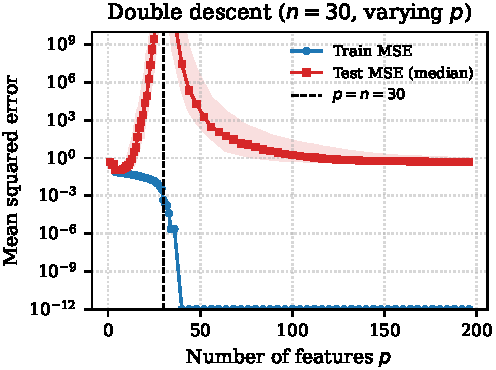
\includegraphics[width=0.55\linewidth]{figures/fig_double_descent.pdf}
\caption{Double descent in least-squares polynomial regression.
With $n=30$ training points, the test error follows the U-shape for
$p<n$, peaks sharply at the threshold $p=n=30$, and \emph{descends a
second time} as the model becomes overparameterised. Solid lines:
medians over $80$ training samples; shading: interquartile range.}
\label{fig:dd}
\end{figure}

The shape is clear. For $p<n$, the test error follows the familiar
U-curve and reaches a small minimum near $p\approx 6$. As $p$
approaches the threshold the test error climbs sharply and reaches a
peak more than \emph{ten orders of magnitude} above the noise floor
at $p=n$. Past the threshold the training error drops to numerical
zero, and the test error \emph{decreases} towards a level only a
little worse than the first descent's minimum. This is the
canonical double-descent shape predicted by recent
theory~\citep{hastie2022surprises} and observed in many other
models~\citep{nakkiran2021deep}.

It is worth pausing on \emph{why} the second descent happens at all.
With $p>n$, infinitely many polynomials fit the data exactly. The
algorithm picks the one with the smallest coefficients, which is the
smoothest available choice. As $p$ grows, the set of admissible
fits gets bigger, and the smoothest one becomes smoother in the
directions that matter, so the test error goes down. Loosely: more
parameters give the algorithm \emph{more room} to find a smooth fit.

\subsection{Bias and variance both blow up at the spike}

Where does the spike at $p=n$ come from? A common informal
explanation is that variance explodes. Some authors instead point
at bias. To settle the question empirically, I split the test error
into squared bias and variance using $400$ independent training
samples (Figure~\ref{fig:bv}).

\begin{figure}[t]
\centering
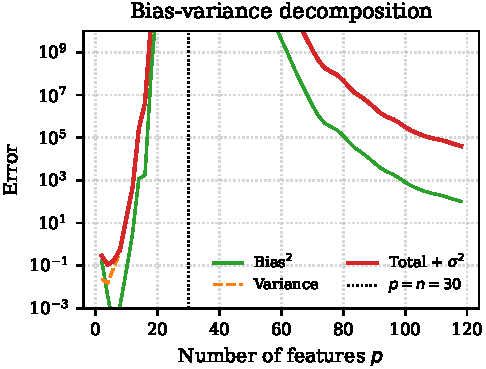
\includegraphics[width=0.55\linewidth]{figures/fig_bias_variance_decomp.pdf}
\caption{Monte Carlo bias--variance decomposition with $n=30$
training points and $400$ independent training samples. \emph{Both}
squared bias and variance peak around the threshold $p=n=30$;
neither alone explains the spike.}
\label{fig:bv}
\end{figure}

The decomposition shows that \emph{both} terms peak around $p=n$.
Squared bias is large near the threshold because the average
prediction (over training samples) is itself an erratic curve
between the training points, far from the smooth target. Variance
is large because tiny changes to the training set lead to wildly
different fits. Both effects come from the same underlying cause:
the design matrix becomes nearly singular at $p=n$. Once $p$ grows
beyond $n$, the design matrix recovers and both terms decay.

\subsection{Ridge regularisation removes the spike}

The minimum-coefficient solution above corresponds to ridge
regression with $\lambda=0$. \citet{nakkiran2020optimal} prove that
with the right amount of ridge, the test error is monotone
decreasing in $p$ and the spike disappears entirely.
Figure~\ref{fig:ridge} reproduces this finding.

\begin{figure}[t]
\centering
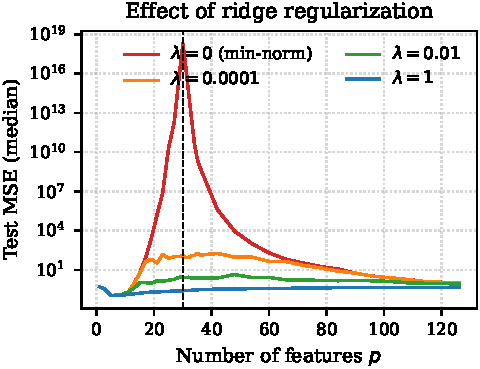
\includegraphics[width=0.55\linewidth]{figures/fig_ridge_regularization.pdf}
\caption{Effect of ridge regularisation on double descent. Even
$\lambda=10^{-2}$ flattens the spike at $p=n$ almost completely;
$\lambda=1$ gives a curve that is essentially monotone in $p$.}
\label{fig:ridge}
\end{figure}

Even a tiny ridge penalty, $\lambda=10^{-4}$, brings the peak down
from about $10^{18}$ to about $10^{1}$. With $\lambda=10^{-2}$ the
curve is essentially flat across the threshold. With $\lambda=1$
the test error is monotone in $p$. This matches the theoretical
prediction of~\citet{nakkiran2020optimal} and gives a useful
practical takeaway: in linear regression, double descent only
appears when there is no explicit regularisation at all.

\section{Discussion}
\label{sec:discussion}

\paragraph{What the experiments do and do not show.} I have
demonstrated double descent in the cleanest setting I could put
together, but the experiments are simple by design. Two limitations
are worth flagging. First, the cleanliness of the curve depends on
a well-behaved basis. The same experiment with raw monomials
produces an unreadable plot dominated by floating-point error.
Second, the setup is one-dimensional, and the smooth wiggly target
in~\eqref{eq:data} can be represented exactly by a sufficiently
large polynomial, so the bias term in the overparameterised regime
decays especially fast. In higher dimensions, or when the target
function does not lie inside the model class, the second descent is
less aggressive~\citep{hastie2022surprises}.

\paragraph{Why this matters in practice.} Two takeaways are worth
keeping in mind. First, the intuition that ``more parameters than
data points'' is automatically pathological is wrong; the
minimum-coefficient solution implicitly regularises and can
generalise just fine. Second, if you suspect you are operating
near the threshold, even a small amount of explicit regularisation
removes the risk of catastrophic test error.

\paragraph{Connection to deep learning.} The phenomenon shown here
in linear regression is closely related, though not identical, to
``model-wise'' double descent in deep neural
networks~\citep{nakkiran2021deep}. In both cases the peak occurs
where the model has just enough capacity to fit the training labels.
In both cases regularisation, early stopping, or more data tends to
mitigate it. The neural-network case has additional sources of
implicit regularisation coming from the optimiser
(e.g.\ stochastic gradient descent), which the linear-regression
analogue does not capture.

\section{Conclusion}
\label{sec:conclusion}

I have given a small, self-contained empirical demonstration of
double descent in least-squares polynomial regression. Three
messages emerge. A well-behaved basis is needed to see the
phenomenon cleanly. The spike at the interpolation threshold
reflects an explosion in \emph{both} bias and variance, not just one
of them. And even a small ridge penalty makes the spike disappear.
I hope this short paper works as a useful pedagogical companion to
the more sophisticated theoretical treatments cited above.

\section*{Reproducibility}

The full source code, the LaTeX sources of this paper, and all the
figures are released as a single archive accompanying this
submission. Each experiment runs in less than a minute on a laptop.
Random seeds are fixed in the script.

\acks{The author thanks the instructors of the Academic Skills in
Computer Science course at Constructor University Bremen for the
opportunity to write this paper. No external funding supported this
work, and the author declares no competing interests.}

\bibliography{refs}

\end{document}
